\section{How does it work?}
\subsection{Attack overview}
\label{subsec:attack_overview}

As mentioned file lockers are the most common ransomware type. An exemplified attack scenario is shown in Figure \ref{fig:attack_scenario}.

\begin{figure}[htbp]
  \begin{center}
    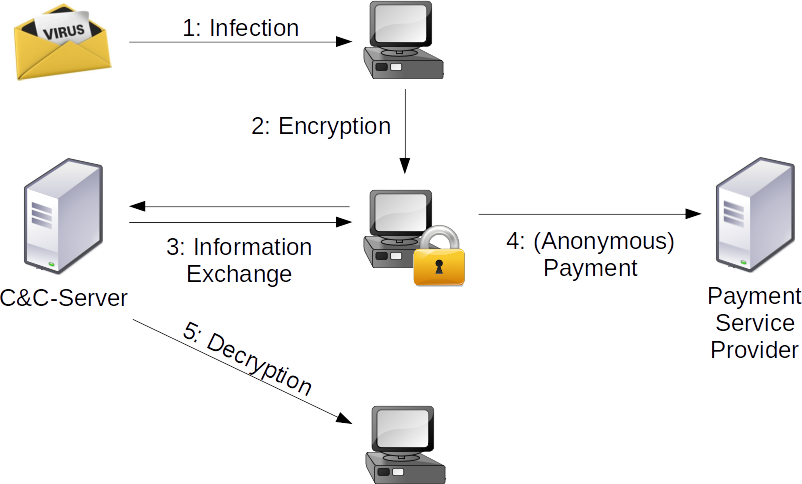
\includegraphics[width=0.8\textwidth]{images/attack_scenario.png}
    \caption{Attack scenario with file lockers}
    \label{fig:attack_scenario}
  \end{center}
\end{figure}

\begin{enumerate}
\item The device of the victim gets infected. Most of the time this happens via mail \cite{OstermanResearch2016}, where it either contains a link to a malicious software or the malicious software is attached directly. \glspl{tds}, malvertisement and social engineering are also used sometimes. Many ransomware variants further infect external storages and devices in the same network.
\item The files of the victim are encrypted. Normally the virus searches for files with specific file endings, which likely are important for the user. For example image file endings like .png and .jpg, as well as Microsoft Word file endings like .doc and .docx are often used. For the encryption itself in recent years well established cryptocraphic standards like AES-128 CBC. The encryption will be discussed in more detail in subsection \ref{subsec:encryption_overview}.
\item The information exchange with the \gls{candc} server. This servers are used to control botnets, but they are also used to communicate with infected devices of ransomware. Often \gls{candc} servers are located in countries with not so stringend law enforcement, so that they can stay alive as long as possible to exchange information with existing and new victims. Usually an unique identifier for every infected device is stored on the server as well as information about the device itself (e.g. number of infected files, infection time etc.). Making contact with a \gls{candc} server can also happen before the encryption, so that unique public/private key pairs are generated for every infected machine.
\item The victim pays the ransom to a payment provider. With the upsurge of crypto currencies like Bitcoin and networks like Tor, it is easier for attackers to stay anonymous when receiving the payment\cite{Liao2016}.
\item The encrypted files of the victim are decrypted. The attacker checks the payment beforehand and initializes the decryption. Therefore the key for the decryption is send to the victim. Some ransomware variants decrypt the files on the \gls{candc} server and send the decrypted files to the victim. Of course there is no gurantee for the victim, that the files are decrypted at all.
\end{enumerate}

As mentioned before this is only an examplified attack scenario. There exist many different variants with different scenarios.

\pagebreak
\subsection{Enryption overview}
\label{subsec:encryption_overview}

In recent years ransomware developers have used both asymmetric and symmetric cryptographic technologies. Figure \ref{fig:encryption_overview} illustrates when these technologies are used.

\begin{figure}[htbp]
  \begin{center}
    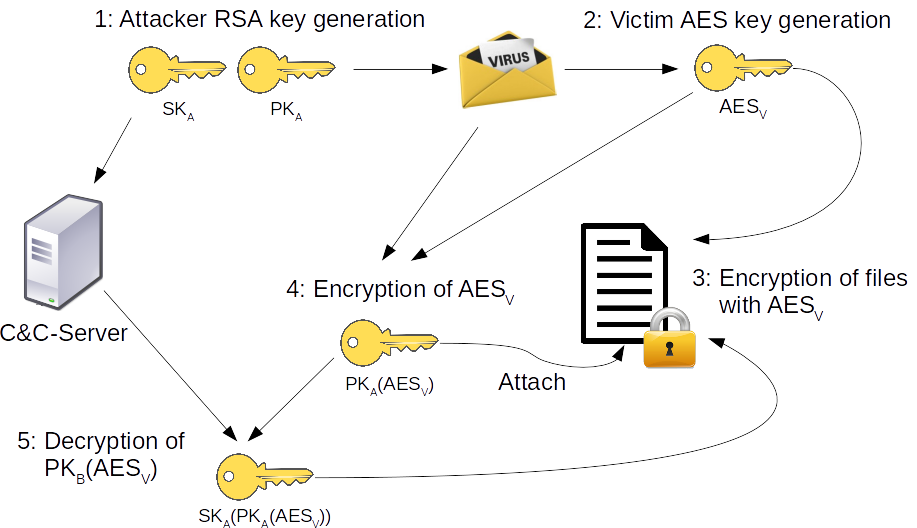
\includegraphics[width=0.8\textwidth]{images/encryption_overview.png}
    \caption{Ransomware encryption overview}
    \label{fig:encryption_overview}
  \end{center}
\end{figure}

\begin{enumerate}
\item The attacker generates and RSA key pair. He stores the secret key $SK_A$ on a \gls{candc} server and includes the public key $PK_A$ in the ransomware. Some ransomware variants create multiple of these key pairs.
\item On the victims device an AES session key $AES_V$ is generated. The generation is triggered by the ransomware on the infected device.
\item The files of the victim are encrypted with the AES session key $AES_V$.
\item The AES session key $AES_V$ is encrypted with the RSA public key $PK_A$. This new key $PK_A(AES_V))$ is often attached to the encrypted files, so that the {candc} server later can decrypt the files by only receiving the files. The AES session key $AES_V$ itself is safely deleted.
\item The key $PK_A(AES_V))$ is decrypted with the secret key $SK_A$. When a decrypted file arrives at the \gls{candc} server, it uses the stored secret key $SK_A$ to decrypt the attached key $PK_A(AES_V)$.\\
With $SK_A(PK_A(AES_V))$ the original AES key $AES_V$ can be restored.
\item The files can be decrypted with the key $AES_V$.
\end{enumerate}
